\chapter{รายละเอียดการปฏิบัติงาน}
\thispagestyle{empty}
\label{chapter:coop-detail}

\section{ตำแหน่ง/หน้าที่ของงานที่ได้รับมอบหมาย}

    \subsection{ตำแหน่งงาน}
        PROGRAMMER
    
    \subsection{หน้าที่ของงานที่ได้รับมอบหมาย}
        \begin{enumerate}
            \item ศึกษาวิธีการทดสอบกับ Flutter แอปพลิเคชันโดยการเพิ่ม key
            \item ศึกษาวิธีการใช้งาน Appium ซึ่งเป็น Framework ที่ช่วยในการทดสอบ แอปพลิเคชัน อัตโนมัติ
            \item ศึกษาวิธีการใช้งาน Appium กับ Flutter ผ่าน Flutter Appium Driver Library
            \item ศึกษาการใช้งาน AWS Device Farm ซึ่งเป็นตัวช่วยจำลองโทรศัพท์ในการทดสอบแอปพลิเคชัน
            \item ศึกษาการพัฒนาชุดคำสั่งทดสอบด้วย NodeJs
            \item ศึกษา HomePro E-Catalog แอปพลิเคชนซึ่งเป็นแอปพลิเคชันที่ต้องนำมาทดสอบ
            \item ออกแบบและพัฒนาชุดคำสั่งทดสอบ
            \item จัดทำคู่มือวิธีการติดตั้ง Appium, AWS Device Farm, NodeJs
            \item จัดทำคู่มือวิธีการพัฒนาชุดคำสั่งทดสอบอัตโนมัติด้วย NodeJs กับ Flutter Appium Driver Library
            \item จัดทำคู่มือวิธีการใช้งาน Appium, AWS Device Farm, NodeJs
        \end{enumerate}

\section{รายละเอียดของโครงงานที่ได้รับผิดชอบ}

    เนื่องจากใน {\Company} เป็นบริษัทขนาดใหญ่จึงจำเป็นต้องมีแอปพลิเคชันหรือระบบภายในไว้ใช้งานจึงมีแผนก ICT Non SAP Front Office
    ไว้คอยพัฒนาระบบหรือแอปพลิเคชันโดยในการจะนำเอาแอปพลิเคชันมาใช้งานหรือแก้ไขต้องเกิดการทดสอบก่อนเสมอเพื่อลดข้อผิดพลาดทางแผนกจึงมอบหมายงาน
    ให้พัฒนาการทดสอบแอปพลิเคชันอัตโนมัติ (Automate Testing) ของแอปพลิเคชัน HomePro E-Catalog ที่เป็นแอปพลิเคชันที่สร้างขึ้นด้วย Flutter เพื่อเป็นต้นแบบไว้คอยนำมาประยุกต์ใช้งานกับ
    แอปพลิเคชันที่จะเกิดขึ้นในอนาคต โดยงานหลักแบ่งได้ 2 อย่างได้แก่
    
    \begin{enumerate}
        \item พัฒนาชุดคำสั่งทดสอบไว้ใช้กับแอปพลิเคชัน HomePro E-Catalog ควบคู่กับ AWS Device Farm
        \item จัดทำเอกสารคู่มือการติดตั้ง, การใช้งาน AWS Device Farm, วิธีการพัฒนาชุดคำสั่งทดสอบ
    \end{enumerate}

    \subsection{ขอบเขตของโครงการ}
        จัดทำชุดคำสั่งทดสอบอัตโนมัติกับแอปพลิเคชันที่ถูกสร้างขึ้นมาด้วย Flutter โดยจะสามารถทดสอบในระบบ Android ได้เท่านั้น โดยกรณีศึกษาจากแอปพลิเคชัน HomePro E-Catalog
        โดยสามรถแบ่งการทดสอบเป็น 34 เหตุการณ์โดยสามารถแบ่งดังนี้
        
        \quad 1. การเขียนทดสอบด้วยกรจับ Element บนหน้าจอโดยไม่ต้องแก้ไขที่ Source Code โดยแบ่งเป็นหน้าจอดังนี้
            \begin{itemize}
                \item หน้าจอ Log-in
                \item หน้าจอ ออกจากระบบ
                \item หน้าจอ รายละเอียดสินค้า
                \item หน้าจอ เปรียบเทียบสินค้า
                \item หน้าจอ รถเข็นสินค้า
                \item หน้าจอ หมวดผู้ใช้งาน
                \item หน้าจอ หมวดเมนู
            \end{itemize}

        \quad 2. การเขียนการทดสอบด้วยการจับ แก้ไขที่ Source Code ของ Flutter โดยใช้ Appium Flutter Driver โดยแบ่งตามหน้าจอดังนี้
            \begin{itemize}
                \item หน้าจอ หมวดสินค้า (Level 3)
                \item หน้าจอ หมวดหมู่ย่อย (Level 2)
                \item หน้าจอ หมวดหมู่ย่อย (Level 1)
            \end{itemize}

        เมื่อพัฒนาชุดคำสั่งเสร็จสิ้นจึงนำไปทดสอบบน AWS Device Farm และจัดทำเอกสารคู่มือวิธีการติดตั้ง, วิธีการพัฒนาชุดคำสั่งทดสอบ, คู่มือการใช้งาน AWS Device Farm

\newpage
\section{รายละเอียดของงานที่ปฏิบัตินอกเหนือจากโครงการที่รับผิดชอบ}
    นอกเหนือจากงานโครงการที่ได้รับผิดชอบยังมีงานอื่นในการช่วยการทำงานของแผนกในฐานะ PROGRAMMER โดยสามารถแบ่งโปรเจ็คที่ได้ทำเป็น 2 ประเภทได้แก่
    
    \subsection{บริการระบบงานขาย Single Sale}
        เป็นระบบที่ใช้ในการยืนยันการซื้อขายสินค้าโดยผู้ใช้งานจะเป็นพนักงานของสาขา {\Company} โดยงานที่ได้รับมอบหมายส่วนใหญ่คือการหาข้อผิดพลาดของระบบและทำการแก้ไข
        ยกตัวอย่าง เช่น การนำข้อมูลออกมาแสดงไม่ถูกต้องจึงต้องไปดูวิธีการนำข้อมูลออกมาและทำการแก้ไขให้ทำงานได้อย่างถูกต้อง หรือ ทำการสร้างหมวดย่อยใหม่เป็นประเภทในการสั่งซื้อสินค้าของลูกค้าเป็นต้น
    
    \subsection{ระบบงานจัดส่งและบริการ Delivery Service}
        เป็นระบบที่ใช้ในการสร้างและยืนยันปิดงานจัดส่งสินค้าโดยผู้ใช้งานจะเป็น พนักงานสาขา, พนักงานจัดส่ง, คอลเซ็นเตอร์ ของ {\Company} โดยงานที่ได้รับมอบหมายส่วนใหญ่คือการหาข้อผิดพลาดของระบบและทำการแก้ไข
        ยกตัวอย่าง เช่น การจัดทีมช่างไปที่บ้านลูกค้าแสดงไม่ถูกต้องจึงต้องทำการแก้ไขให้แสดงได้อย่างถูกต้อง หรือ การปิดงานบางครั้งเป็นงานต่อเนื่องทำหลายวัน
        แต่ระบบได้ปิดงานไปแล้วจึงต้องทำการแก้ไขให้สามารถเก็บการปิดงานเป็นรายวันได้

\section{ลักษณะขั้นตอนกํารทำงาน}
        ลักษณะขั้นตอนการทำงานเป็น รูปแบบ WaterFall มี step การทำอย่างชัดเจนโดยสามารถแบ่งการทำงานดังนี้
        \begin{enumerate}
            \item ศึกษาแอปพลิเคชันที่ต้องการนำมาทดสอบ
            \item ศึกษาวิธีการพัฒนาชุดคำสั่งทดสอบอัตโนมัติ
            \item พัฒนาชุดคำสั่งทำสอบอัตโนมัติแล้วนำไปทดสอบบน AWS Device Farm
            \item จัดทำคู่มือวิธีการติดตั้ง, จัดทำคู่มือวิธีการพัฒนาชุดคำสั่งทดสอบอัตโนมัติด้วย, จัดทำคู่มือวิธีการใช้งาน
            \item รายงานผลการทดลอง
            \item ส่งมอบชุดคำสั่งทดสอบ
        \end{enumerate}


\section{ทฤษฎีที่เกี่ยวข้อง}
    \subsection{การทดสอบซอฟต์แวร์ (Software Testing)}
        Software Testing คือ การทดสอบว่าระบบทำงานได้อย่างถูกต้องหรือไม่ตามวัตถุประสงค์หรือเปล่าและสามารถระบุข้อผิดพลาดเพื่อสามารถนำไปแก้ไขได้
        ก่อนการนำไปจัดส่งซึงการทำการทดสอบซอฟต์แวร์นั้นมีความสำคัญมากเนื่องจากการเจอ ข้อผิดพลาดในซอฟต์แวร์นั้นมีค่าใช้จ่ายที่สูงหากเกิดขึ้นตอนนำจัดส่งไปแล้ว
        โดยการทดสอบซอฟต์แวร์แบ่งเป็นได้ 2 ประเภทได้แก่
        \begin{enumerate}
            \item Manual Testing คือ การทดสอบที่ไม่ใช้เครื่องมืออัตโนมัติหรือ Script เลยจะทดสอบตาม Test Plan, Test Case หรือ Test Scenarios ด้วยมือของผู้ทดสอบเอง
            \item Automation Testing คือ การทดสอบอัตโนมัติด้วยการเขียนชุดคำสั่งในการทดสอบ (Script)
        \end{enumerate}
        \begin{figure}[H]
            \centering
            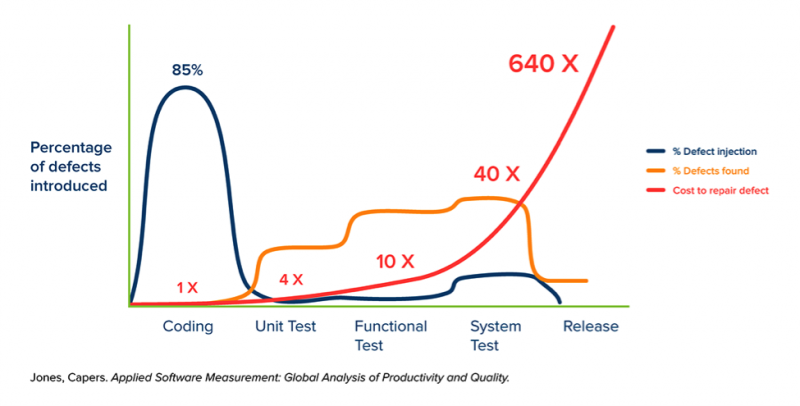
\includegraphics[width=1\textwidth]{cost-of-fixing-bug}
            \caption{ค่าใช้จ่ายการแก้ข้อผิดพลาดที่แปรผันตามขั้นตอนของการพัฒนาซอฟต์แวร์}\label{cost-of-fixing-bug}
        \end{figure}

    \subsection{การทดสอบอัตโนมัติ (Automation Testing)}
        Automation Testing คือ การทดสอบแบบอัตโนมัติโดยการเขียนชุดคำสั่งทดสอบแทนแบบเดิมที่ใช้การทดสอบก้วยมือ ยกตัวอย่าง เช่น
        การทดสอบซอฟต์แวร์แบบเดิมด้วยการใช้มือจะต้องกรอกแบบสอบถามในแอปพลิเคชันในวันแรกและเจอข้อผิดพลาดวันถัดไปนักพัฒนาแอปพลิเคชัน
        ก็ปรับปรุงแอปพลิเคชันมาใหม่ให้ไปทดสอบกรอกแบบเดิมอีกและอาจเจอข้อผิดพลาดใหม่หรือไม่เจอแต่ถ้าหากเกิดการแก้ไขหรือเปลี่ยนแปลงกับ
        ตัวแอปพลิเคชันแล้วต้องทำการทดสอบใหม่อยู่ตลอดซึ่งเป็นการทำงานรูปแบบเดิม แต่การทำ Automation Testing จะมาช่วยแก้ปัญหาโดย
        การเขียนชุดคำสั่งเพื่อมากรอกแบบทดสอบให้ในแอปพลิเคชันซึ่งกำหนดไว้ว่าสิ่งที่ถูกต้องควรจะเป็นอย่างไรและหากไม่ถูกต้องไม่ถูกต้องอย่างไร
        โดยจะเป็นการทำแบบอัตโนมัติด ดังนั้นข้อดีของ Automation Testing ได้แก่
        \begin{itemize}
            \item[-] ผลตอบรับที่ไวขึ้นต่อรอบการพัฒนาหรือแก้ไขแอปพลิเคชัน
            \item[-] สามารถประหยัดค่าใช้จ่ายในการทดสอบได้
            \item[-] สามารถทดสอบได้อย่างคลอบคลุมมากขึ้น
            \item[-] สามารถนำแอปพลิเคชันมาส่งมอบได้เร็วขึ้น
            \item[-] เพิ่มความแม่นยำในการทดสอบมากขึ้น 
            \item[-] กำจัดการทดสอบที่จะผิดพลาดที่เกิดจากมนุษย์ 
        \end{itemize}
        ในปัจจุบันมีเครื่องมือช่วยในการทำ Automation Testing มากมายยกตัวอย่างดังนี้
        \begin{enumerate}

            \item Katalon Studio คือ เครื่องมือตัวหนึ่งในการช่วยทำ Test Automation ของ Mobile Applications ซึ่งสามารถทดสอบได้ทั้ง
            Android และ IOS
            \begin{figure}[H]
                \centering
                
\includegraphics[width=0.3\textwidth]{katalon-studio}
                \caption{ตราตราสัญลักษณ์ Katalon Studio}\label{katalon-studio}
            \end{figure}

            \item Selenium คือ Software Testing Framework ที่มีประสิทธิภาพไว้ใช้สำหรับเขียนชุดคำสั่งทดสอบ Web Applications ซึ่งเป็นแบบ Open Source สามารถเขียนได้ด้วยหลายภาษา เช่น Java, Python, \texttt(C\#), Javascript, PHP, Perl 
            \begin{figure}[H]
                \centering
                
\includegraphics[width=0.5\textwidth]{selenium}
                \caption{ตราตราสัญลักษณ์ Selenium}\label{selenium}
            \end{figure}

            \item Micro Focus UFT คือ หนึ่งใน Software ที่มีประสิทธิภาพที่สุดสำหรับการทำการทดสอบแบบ Functional Testing สามารถสร้าง Test และแก้ไขได้อย่างรวดเร็วไปจนถึงสามารถนำเทคโนโลยี Object Recognition, Image-based Automation และ Machine Driven Regression Testing เข้ามาใช้ช่วยในการทำงาน
            แต่เสียค่าใช้จ่ายแต่มีให้ทดลองใช้งานฟรี 60 วัน
            \begin{figure}[H]
                \centering
                
\includegraphics[width=0.20\textwidth]{uft}
                \caption{ตราตราสัญลักษณ์ Micro Focus UFT}\label{uft}
            \end{figure}

            \item TestComplete คือ หนึ่งใน Software ที่มีประสิทธิภาพที่สุดสำหรับการทำการทดสอบ Desktop, Mobile และ Web Applications ตามชุดคำสั่งที่เขียนได้ด้วย
            ภาษา Python, JavaScript, VBScript และอื่นๆ
            \begin{figure}[H]
                \centering
                
\includegraphics[width=0.5\textwidth]{test-com}
                \caption{ตราตราสัญลักษณ์ TestComplete}\label{test-com}
            \end{figure}


        \end{enumerate}

    \subsection{Appium}
        Appium คือ เครื่องมือสำหรับการทำ Automation Testing เป็นรุปแบบ Open Source ไว้สำหรับทดสอบ Native, Mobile Web, Hybrid
        , Android, IOS และ Windows Desktop การใช้ Appium จะเป็น Cross Platform หมายความว่าจะทำให้สามารถเขียน
        โดยใช้ API เดียวกันซึ่งจะช่วยให้สามารถใช้โค้ดซ้ำระหว่างอุปกรณ์ที่ทดสอบได้ IOS, Android, Window การทำงานจะสื่อสารระหว่าง Driver กับ Appium ผ่าน JSON โดยรองรับการเขียนได้หลายภาษา
        เช่น Python, Java, JavaScript(NodeJS), Ruby 
        \begin{figure}[H]
            \centering
            
\includegraphics[width=0.3\textwidth]{appium}
            \caption{ตราตราสัญลักษณ์ Appium}\label{appium}
        \end{figure}

        Driver ที่สามารถใช้กับ Appium ได้แก่
        \begin{itemize}
            \item XCUITest Driver (for iOS and tvOS apps)
            \item Espresso Driver (for Android apps)
            \item UiAutomator2 Driver (for Android apps)
            \item Windows Driver (for Windows Desktop apps)
            \item Mac Driver (for Mac Desktop apps)
        \end{itemize}

        \begin{figure}[H]
            \centering
            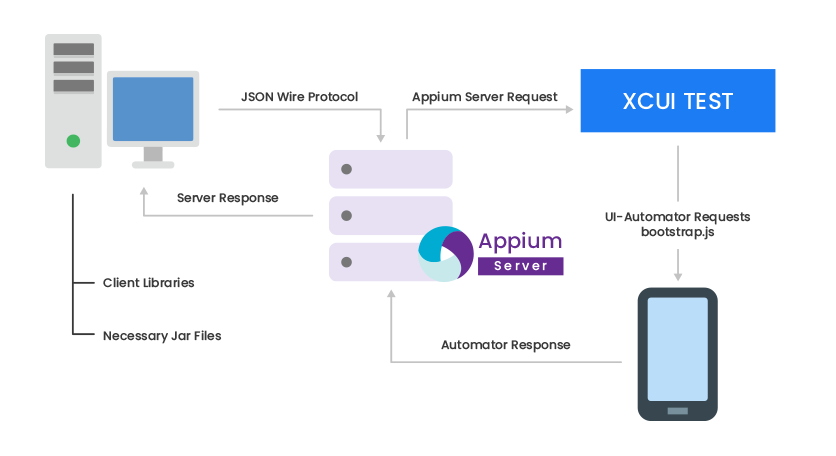
\includegraphics[width=1\textwidth]{appium-arc}
            \caption{โครงสร้างการทำงานของ Appium}\label{appium-arc}
        \end{figure}

        นอกเหนือจากนี้ Appium ยังสามารถใช้งานร่วมกับ AWS Device Farm ได้

    \subsection{API}
        API (Application Programming Interface) คือ วิธีการติดต่อสื่อสารระหว่างแอปพลิเคชันไม่ว่าแอปพลิเคชันนั้นจะรันอยู่บนอุปกรณ์ใด เช่นคอมพิวเตอร์ โทรศัพท์มือถือ หรือเฟิร์มแวร์ในอุปกรณ์เครื่องใช้ต่างๆ โดยที่แอปพลิเคชันฝั่งหนึ่งเป็นผู้ขอใช้บริการหรือขอข้อมูลจากแอปพลิเคชันอีกฝั่งหนึ่งซึ่งเป็นผู้ให้บริการ การติดต่อสื่อสารระหว่างแอปพลิเคชันดังกล่าวเป็นไปโดยอัตโนมัติตามที่ได้กำหนดไว้

    \subsection{AWS Device Farm}
         AWS คือ Amazon Web Services เป็นคลาวด์แพลตฟอร์มที่มีคนนำมาใช้มากที่สุดในโลกที่มีการบริการ 175 บริการ
         โดยองค์กรขนาดใหญ่หรือสตาร์ทอัพก็เริ่มหันมาใช้ AWS เพื่อลดค่าใช้จ่ายและความคล่องตัว

        \begin{figure}[H]
            \centering
            
\includegraphics[width=0.5\textwidth]{aws}
            \caption{ตราสัญลักษณ์ Amazon Web Service (AWS)}\label{aws}
        \end{figure}

        AWS Device Farm คือ บริการหนึ่งของ AWS เป็นบริการไว้ทดสอบแอปพลิเคชันเพื่อปรับปรุงคุณภาพแอปพลิเคชันหรือระบบต่างๆ
        โดย AWS Device Farm จะทดสอบแอปพลิเคชันหรือระบบใน Desktop, Browser หรืออุปกรณ์มือถือที่หลากหลายทั้งในระบบปฎิบัติการ Android และ IOS พร้อมกันเพื่อช่วย
        ให้ชุดทดสอบรวดเร็วขึ้น หลากหลายมากขึ้น และพร้อมสร้างวีดีโอและบันทึกเพื่อช่วยให้หาปัญหาของระบบหรือแอปพลิเคชันได้ไวยิ่งขึ้น

        \begin{figure}[H]
            \centering
            
\includegraphics[width=0.25\textwidth]{amazon-device-farm}
            \caption{ตราสัญลักษณ์ AWS Device Farm}\label{amazon-device-farm}
        \end{figure}

    \subsection{Node.Js}
        Node.Js คือ JavaScript runtime environment เป็น OpenSource คือการที่สามารถนำเอา JavaScript มาใช้งานแบบภาษาอื่นบน
        Windows, Linux หรือ Mac ได้แบบไม่เสียค่าใช้จ่ายหากติดตั้ง Node.js จะสามารถเขียนโปรแกรมด้วยภาษา JavaScript เหมือนกับ Java, \texttt(C\#), Python
        ซึ่งหลักๆแล้วจะนำมาทำเป็น backend server นอกจากนี้ Node.Js ยังมี NPM (Node Package Manager) เป็นตัวที่ใช้สำหรับการดาวน์โหลด
        library ภายนอกมาใช้โดยติดตั้งเพียงพิมพ์ `npm install <ชื่อ library>` เช่น mocha, express, chai เป็นต้น

        \begin{figure}[H]
            \centering
            
\includegraphics[width=0.3\textwidth]{node}
            \caption{ตราสัญลักษณ์ Node.JS}\label{node}
        \end{figure}
        

    \subsection{Flutter}
        Flutter คือ Framework แบบ OpenSource ที่ถูกพัฒนาโดย Google มีไว้เพื่อใช้สร้าง UserInterface สำหรับ Mobile Application ที่สามารถทำงานข้ามแพลตฟอร์มได้ทั้ง IOS และ Android คือเขียนโปรแกรมหนึ่งครั้งสามารถนำมาใช้ได้ทั้งสองแพลตฟอร์มโดยภาษาที่ Flutter ใช้คือภาษา Dart
        โดยจุดเด่นของ Flutter คือระบบ Hot Reload จะเข้ามาช่วยในส่วนของการ reload สามารถพัฒนาแอปพลิเคชัน ในส่วน UserInterface มีความรวดเร็วมากขึ้นอีกทั้งยังมีความสวยงามแบบ
        Material Design

        \begin{figure}[H]
            \centering
            
\includegraphics[width=0.5\textwidth]{flutter}
            \caption{ตราสัญลักษณ์ Flutter}\label{flutter}
        \end{figure}

    \subsection{Appium Flutter Driver}
        Appium Flutter Driver คือ เครื่องมือช่วยในการทำ Automation Test กับแอปพลิเคชันที่สร้างมาจาก Flutter เป็นส่วนหนึ่งในการใช้งานกับ Appium โดย Appium Flutter Driver จะใช้ Dart Service Protocol เพื่อส่ง API ไปเรียกใช้การ Test ของ Flutter ที่ทั่วไปต้องเขียนเป็นภาษา Dart แต่ถ้าใช้ library นี้จะเขียนภาษาตามที่ Appium มีได้เลย

        \begin{figure}[H]
            \centering
            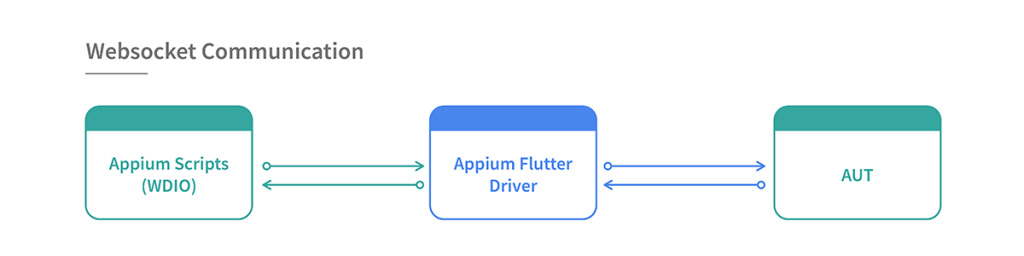
\includegraphics[width=1\textwidth]{appium-flutter}
            \caption{โครงสร้างการทำงานของ Appium Flutter Driver}\label{appium-flutter}
        \end{figure}

    \subsection{"Wd"}
        Wd คือ library JavaScript ที่ใช้ในการทำ Automation Test ใน NodeJS โดยที่สามารถทำงานร่วมกับ Selenium และ Appium ใช้จับ element แบบ xpath

    \subsection{WebdriverIO}
        WebdriverIO คือ library JavaScript ที่ใช้ในการทำ Automation Test ใน NodeJS โดยที่สามารถทำงานร่วมกับ Selenium และ Appium ได้

    \subsection{Xpath}
        Xpath คือ ตัวชี้ทางในภาษาต่างๆ (เช่น XML, HTML) เพื่อแสดง Root ของเส้นทางการเข้าถึงข้อมูลตามลำดับชั้น
        
    \subsection{Mocha}
        Mocha คือ library JavaScript ที่ใช้ใน NodeJs เพื่อทำการทดสอบอัตโนมัติแบบ Asynchronous Testing ได้ง่ายขึ้นโดยการแสดงผลลัพธ์ที่ผิดพลาดอย่างง่ายและชัดเจนตาม Test Case

    \subsection{Chai}
        Chai คือ library JavaScript ที่ใช้ใน NodeJs ทำหน้าที่เปรียบที่ค่าผลลัพธิ์ที่ได้จากการทดสอบกับผลลัพธ์ที่ควรจะเป็นโดยเป็นรูปแบบที่เข้าใจง่าย

    \subsection{Git}
        Git คือ Vesion Control เป็นตัวที่ใช้จัดเก็บและคอยดูการเปลี่ยนแปลงกับไฟล์ชนิดใดก็ได้เมื่อจัดเก็บไฟล์เข้าไปในระบบของ Git แล้วจะเรียกว่า Git Repository ซึ่งสำรองข้อมูลของ Source Code สามารถย้อนกลับไปเวอร์ชั่นใดก่อนหน้าและดูรายละเอียดการเปลี่ยนแปลงของแต่ละเวอร์ชั่นได้

        \begin{figure}[H]
            \centering
            
\includegraphics[width=0.3\textwidth]{git-logo}
            \caption{ตราสัญลักษณ์ Git}\label{git-logo}
        \end{figure}

    \subsection{Visual Studio Code}
        Visual Studio Code คือ Editor ตัวหนึ่งที่สร้างมาเพื่ออำนวยความสะดวกแก่โปรแกรมเมอร์มีธีมและรองรับรูปแบบการเขียนได้หลายภาษาอีกทั้งยังมีตัวช่วยในการเขียนโปรแกรมต่างๆ เช่น Bracket Matcher, Live Server เป็นต้น

        \begin{figure}[H]
            \centering
            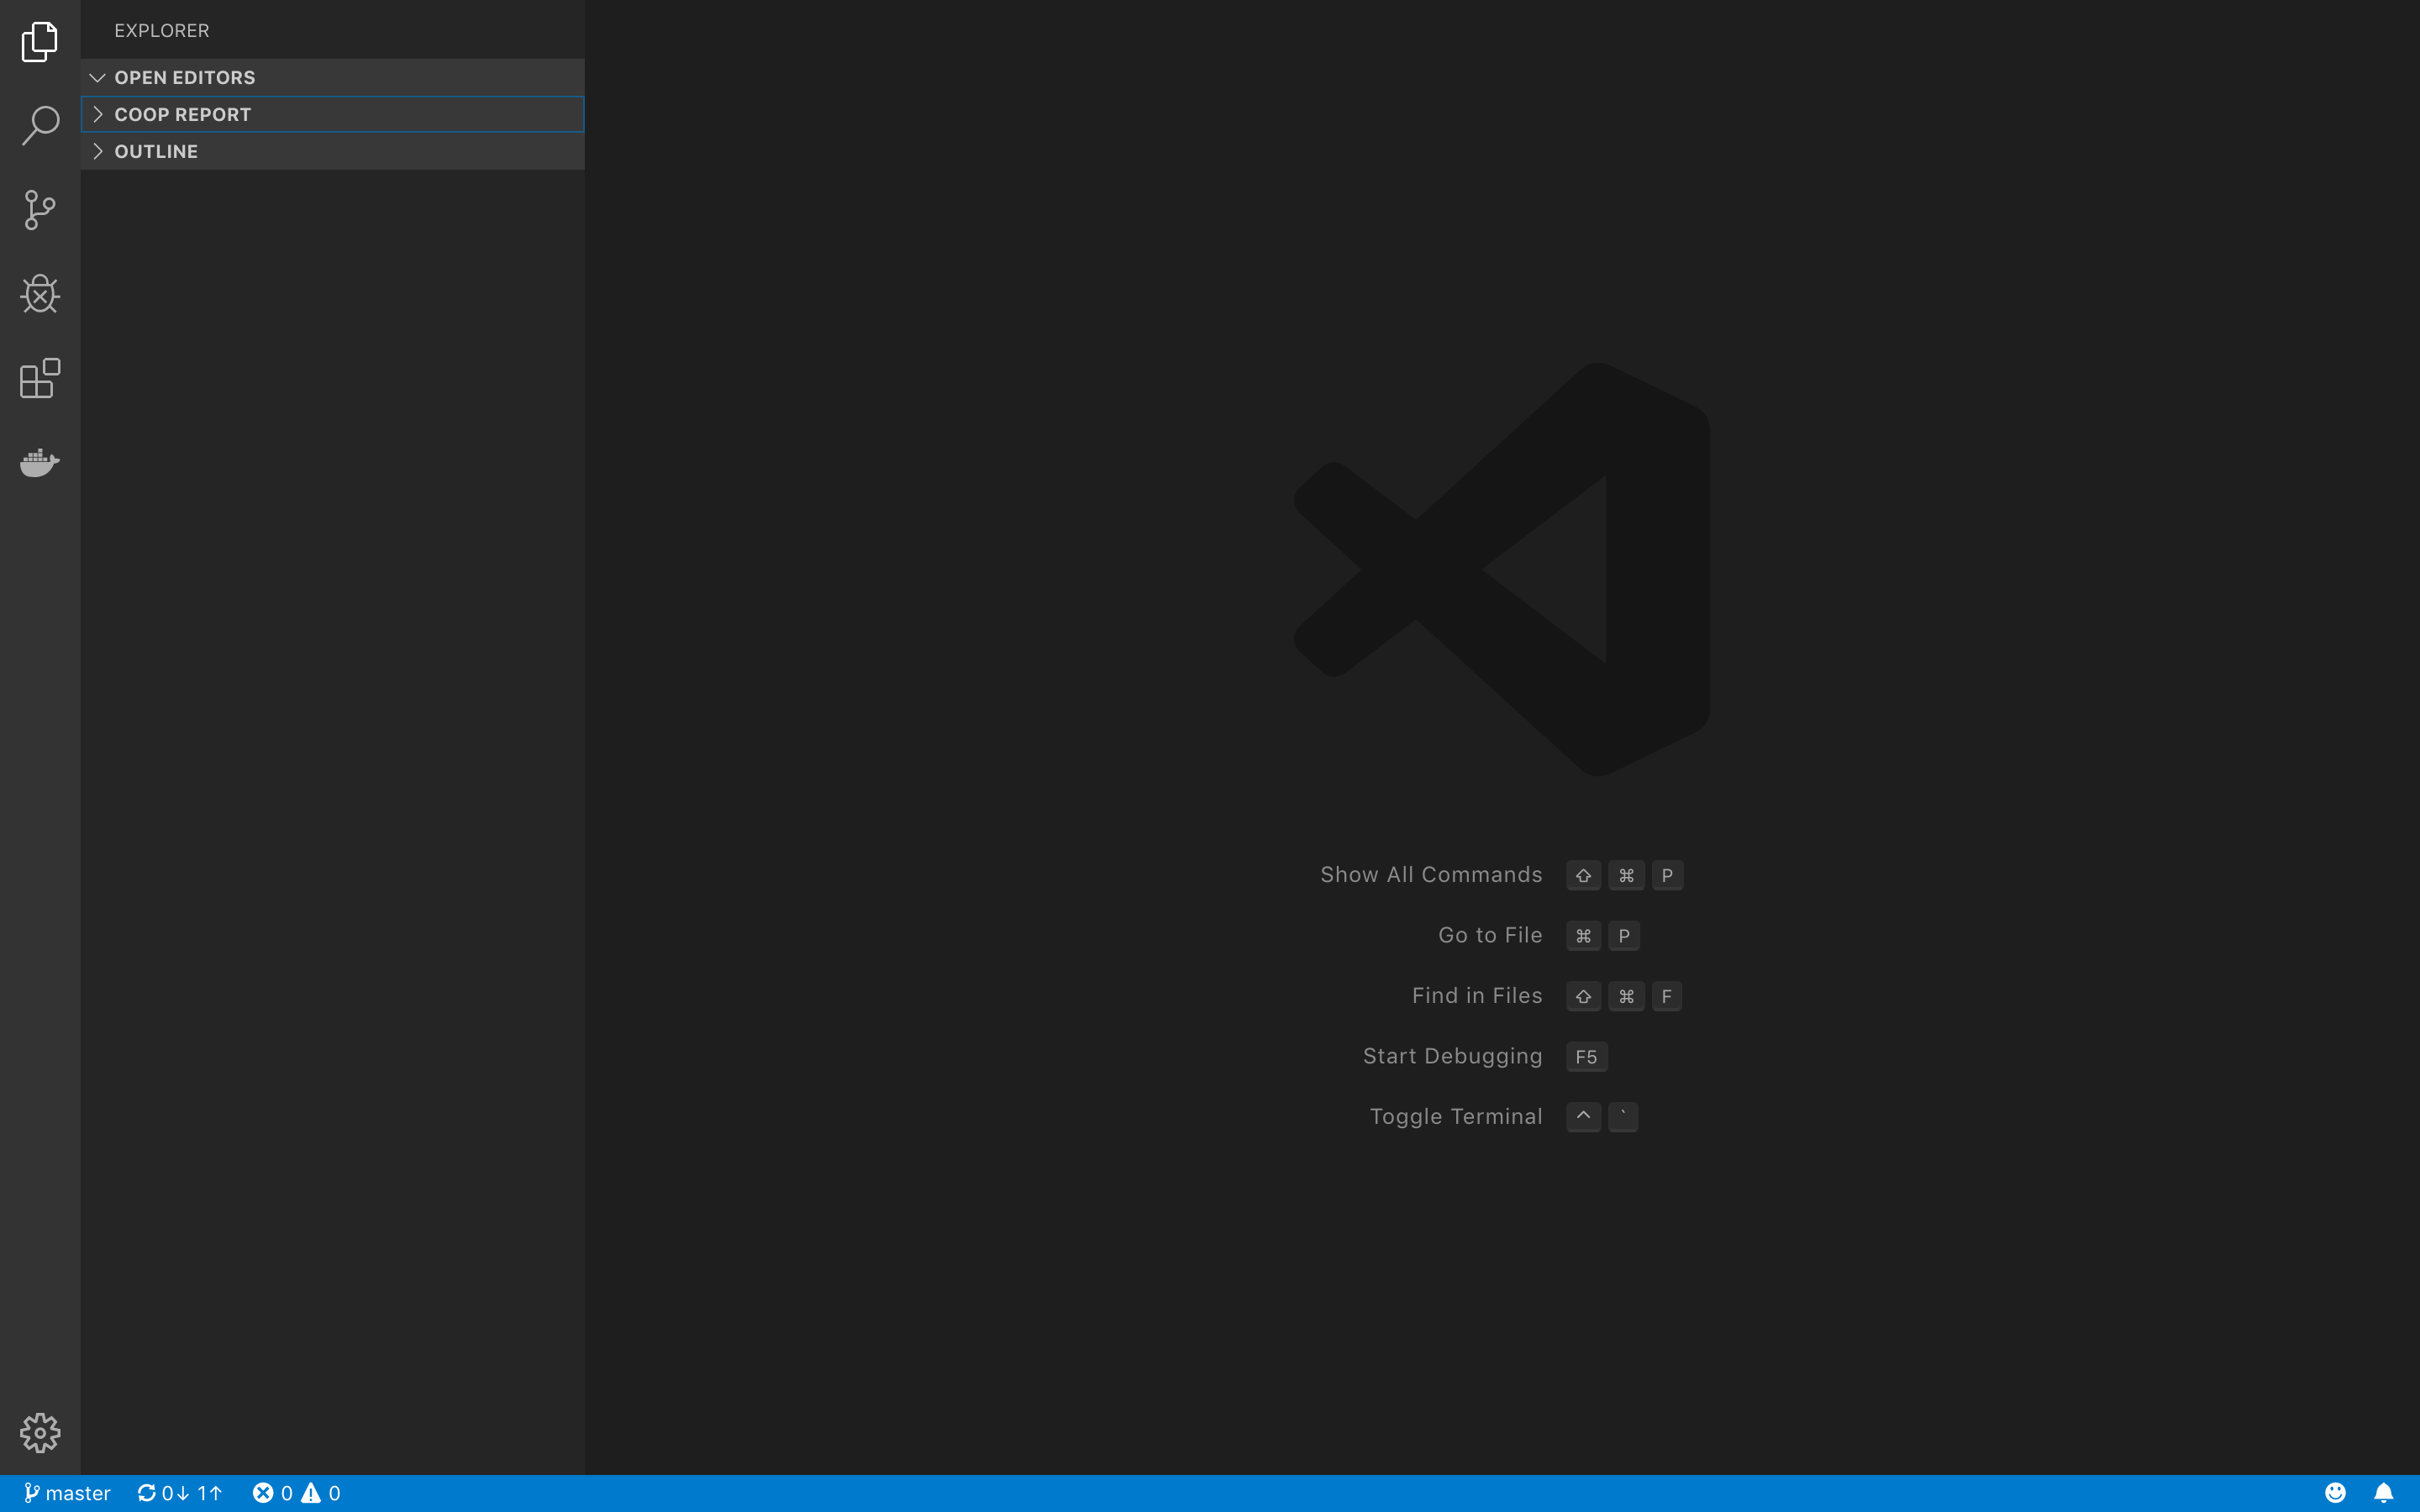
\includegraphics[width=0.2\textwidth]{visual-studio-code}
            \caption{ตราสัญลักษณ์ Visual Studio Code}\label{visual-studio-code}
        \end{figure}